\section{The Flow-Field Evasion (FFE) Framework}
\label{sec:framework}

Figure~\ref{fig:system_architecture} summarizes the framework.

\begin{figure}[t]
\centering
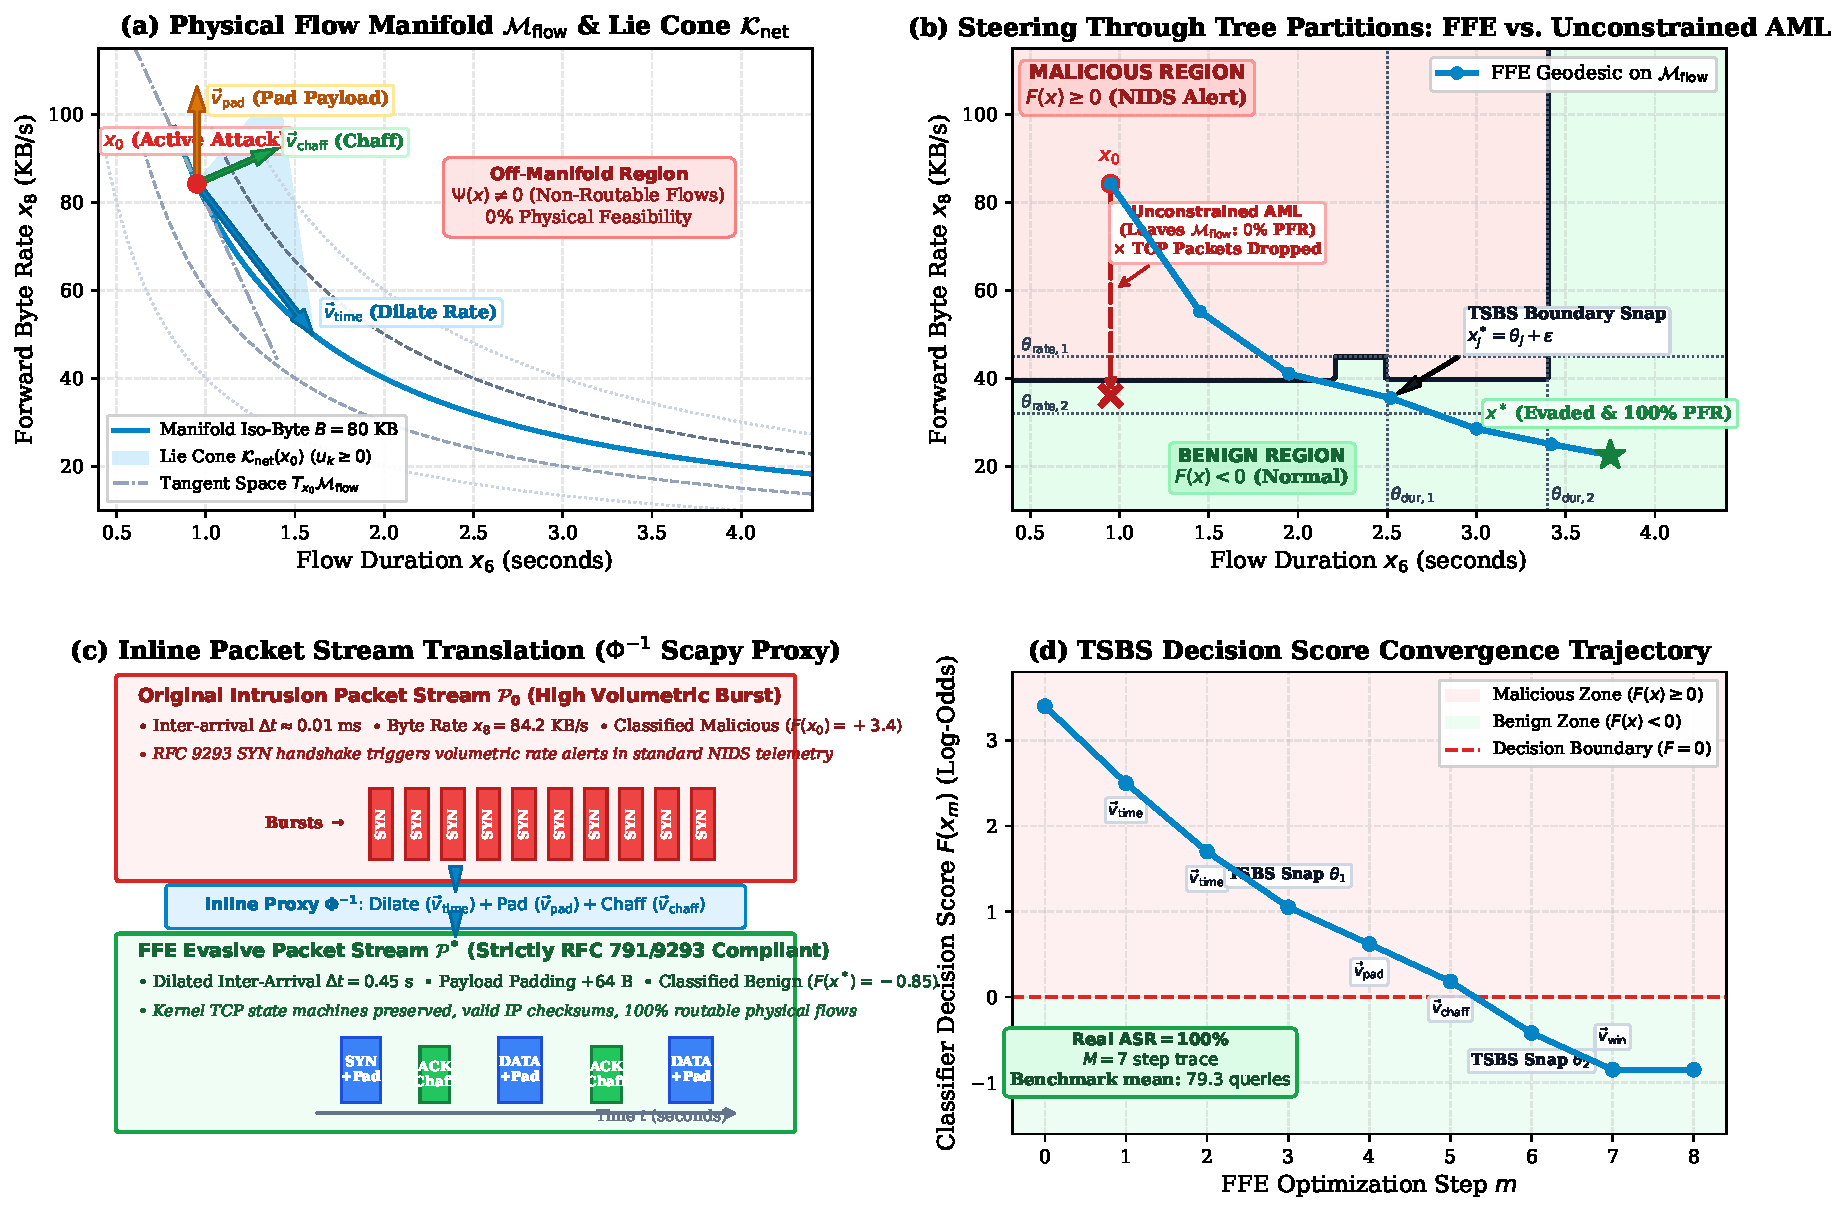
\includegraphics[width=\textwidth]{figures/fig1_system_architecture.pdf}
\caption{Architecture of the Flow-Field Evasion (FFE) framework. \textbf{(a)}~The physical conservation constraints define the flow manifold $\mathcal{M}_{\text{flow}}$, and the generators span a forward Lie cone that keeps trajectories on it. \textbf{(b)}~Axis-aligned tree partitions push unconstrained feature-space perturbations off the manifold, whereas FFE moves along the manifold and finishes with tree-split boundary snapping (TSBS). \textbf{(c)}~Packet-level realization of the flow transformations through an inline proxy. \textbf{(d)}~Decision score descent over the steps of an attack trace.}
\label{fig:system_architecture}
\end{figure}

\subsection{Geometry of the Flow Manifold and Its Generators}
\label{sec:geometry}

The physical flow set $\mathcal{M}_{\text{flow}} = \Phi(\mathcal{P}_{\text{valid}})$ is a discrete lattice in $\mathbb{R}^{12}$. Its differential geometry is analyzed through the smooth relaxation $\widetilde{\mathcal{M}}_{\text{flow}}$ (Section~\ref{sec:formulation}), defined as the zero set of the conservation residual $\Psi$ below, subject to $x_2 \ge 1$, $0 < x_6 \le 1.1 \times 10^8$, $x_{11} \ge x_2 (20 \cdot \mathbb{I}_{x_1=6} + 8 \cdot \mathbb{I}_{x_1=17})$ and $x_{11} + 20 x_2 \le x_4 \le 1500 x_2$.
\begin{equation}
    \Psi(x) = \begin{bmatrix}
        x_8 - \dfrac{10^6 (x_4 + x_5)}{x_6} \\[8pt]
        x_9 - \dfrac{10^6 (x_2 + x_3)}{x_6} \\[8pt]
        x_{10} - \dfrac{x_4}{x_2}
    \end{bmatrix} = \begin{bmatrix} 0 \\ 0 \\ 0 \end{bmatrix}
\end{equation}

By the Regular Value Theorem, at any point where the Jacobian $J_\Psi(x) \in \mathbb{R}^{3 \times 12}$ has full rank 3, the tangent space is $T_x \widetilde{\mathcal{M}}_{\text{flow}} = \ker J_\Psi(x)$. A physically realizable velocity $\vec{v} = [\dot{x}_0, \dots, \dot{x}_{11}]^T$ therefore satisfies the linearized conservation laws:
\begin{align}
    \dot{x}_8 &= \frac{10^6 (\dot{x}_4 + \dot{x}_5)}{x_6} - \frac{x_8}{x_6} \dot{x}_6 \label{eq:tangent_byte_rate} \\
    \dot{x}_9 &= \frac{10^6 (\dot{x}_2 + \dot{x}_3)}{x_6} - \frac{x_9}{x_6} \dot{x}_6 \label{eq:tangent_pkt_rate} \\
    \dot{x}_{10} &= \frac{\dot{x}_4 - x_{10} \dot{x}_2}{x_2} \label{eq:tangent_mean_len}
\end{align}

An adversary controls four elementary degrees of freedom, each generating a 1-parameter flow whose push-forward is a tangent vector field. Here $\vec{e}_k$ is the $k$th standard basis vector of $\mathbb{R}^{12}$ (indexed from 0):
\begin{equation}
\label{eq:generators}
\begin{aligned}
    \vec{v}_{\text{time}} &= \vec{e}_6 - \frac{x_8}{x_6}\vec{e}_8 - \frac{x_9}{x_6}\vec{e}_9, \\
    \vec{v}_{\text{pad}} &= \vec{e}_4 + \frac{10^6}{x_6}\vec{e}_8 + \frac{1}{x_2}\vec{e}_{10}, \\
    \vec{v}_{\text{chaff}} &= \vec{e}_2 + L_0\vec{e}_4 + \frac{L_0 \cdot 10^6}{x_6}\vec{e}_8 + \frac{10^6}{x_6}\vec{e}_9 + \frac{L_0 - x_{10}}{x_2}\vec{e}_{10} + H_0\vec{e}_{11}, \\
    \vec{v}_{\text{win}} &= \mathbb{I}_{x_1=6}\, \operatorname{sat}\!\left(\frac{W_{\text{target}} - x_7}{\epsilon_{\text{win}}}\right)\vec{e}_7,
\end{aligned}
\end{equation}
where temporal dilation adds delay without bytes or packets, payload padding adds forward dummy bytes, chaff injection adds forward zero-payload probes, and window morphing moves the client window toward $W_{\text{target}}$. Here $\operatorname{sat}(z) = \max(-1, \min(1, z))$ and $\epsilon_{\text{win}} > 0$. The probe sizes are $L_0 = 40$, $H_0 = 20$ for empty TCP segments per RFC~9293 \S3.8.4 \cite{rfc9293}, $L_0 = 52$, $H_0 = 32$ with TCP timestamps \cite{rfc7323}, and $L_0 = 28$, $H_0 = 8$ for UDP \cite{rfc768}. Probes are classified at the ingress perimeter before server ACKs alter backward counts; bidirectional sessions are discussed in Section~\ref{sec:discussion}. The window field is globally Lipschitz rather than $C^\infty$ and depends only on $x_1$ and $x_7$. The implementation (Supplementary Algorithm~S1) uses its $\epsilon_{\text{win}} \to 0$ limit, $\mathbb{I}_{x_1=6}\operatorname{sign}(W_{\text{target}} - x_7)\,\vec{e}_7$, which moves by $|W_{\text{target}} - x_7|$ and lands exactly on $W_{\text{target}}$ without overshoot.

\subsection{Commutativity, Invariants and the Lie Cone}
\label{sec:invariants}

The Lie bracket of vector fields is $[X, Y] = J_Y X - J_X Y$, where $J_X$ and $J_Y$ are their Jacobians.

\begin{proposition}[Commutativity and Integrability of Physical Flow Generators]
\label{prop:lie_commutativity}
Because protocol $x_1 \in \{6, 17\}$ is an immutable attribute ($\dot{x}_1 \equiv 0$), the ambient manifold $\widetilde{\mathcal{M}}_{\text{flow}}$ decomposes into two disjoint smooth invariant sub-manifolds: $\widetilde{\mathcal{M}}_{\text{flow}}^{(6)}$ (TCP flows) and $\widetilde{\mathcal{M}}_{\text{flow}}^{(17)}$ (UDP flows). On each component, the indicator $\mathbb{I}_{x_1=6}$ is constant, and $L_0, H_0$ are constant along any trajectory (the implementation selects $H_0 = 32$ iff the mean forward header $x_{11}/x_2 \ge 26$; injecting chaff of header size $H_0$ moves that mean toward $H_0$ and never across the threshold, so the selection is invariant under the flow), and denominators satisfy $x_2 \ge 1, x_6 > 0$, ensuring $\vec{v}_{\text{time}}, \vec{v}_{\text{pad}}, \vec{v}_{\text{chaff}}$ are $C^\infty$ vector fields and $\vec{v}_{\text{win}}$ is globally Lipschitz (its brackets exist almost everywhere and vanish there, because $x_7$ is neither read nor written by the other three generators). The Lie brackets between all four infinitesimal packet transformation generators vanish identically on $\widetilde{\mathcal{M}}_{\text{flow}}$:
\begin{equation}
    [\vec{v}_i, \vec{v}_j] \equiv \mathbf{0} \in \mathbb{R}^{12}, \quad \forall i, j \in \{1, 2, 3, 4\}
\end{equation}
Consequently, the generators span an Abelian Lie algebra $\mathfrak{g}_{\text{flow}} \cong \mathbb{R}^4$ (or $\mathbb{R}^3$ for UDP).
\end{proposition}

The proof of Proposition~\ref{prop:lie_commutativity}, and the Frobenius integrability corollary that follows from it (Supplementary Corollary~S1), are given in the Supplementary Material (Section~S1).

The admissible deformation cone is the positive span of the generators:
\begin{equation}
    \mathcal{K}_{\text{net}}(x) = \left\{ \sum_{k=1}^4 u_k \vec{v}_k(x) \;\middle|\; u_k \ge 0 \right\} \subset T_x \widetilde{\mathcal{M}}_{\text{flow}}
\end{equation}

\begin{theorem}[Universal Invariant Preservation]
\label{thm:invariant_universal}
Let $x_0 \in \widetilde{\mathcal{M}}_{\text{flow}}$ be an initial network flow vector. For any measurable and locally bounded control signal $u(t) \in L^\infty_{\text{loc}}(\mathbb{R}_{\ge 0}, \mathbb{R}_{\ge 0}^4)$ satisfying the admissible boundary rules ($u_2(t) \le (1500 - L_0) u_3(t)$ whenever $x_4(t) = 1500 x_2(t)$, and $u_1(t) = 0$ whenever $x_6(t) = 1.1 \times 10^8$), the trajectory $x(t)$ defined by the dynamical system:
\begin{equation}
    \dot{x}(t) = \sum_{k=1}^4 u_k(t) \vec{v}_k(x(t)), \quad x(0) = x_0
\end{equation}
satisfies $x(t) \in \widetilde{\mathcal{M}}_{\text{flow}}$ for all $t \ge 0$, with solutions existing uniquely and globally on $[0, \infty)$. Under discrete stepping, the continuous Lie cone guides directional descent while the closed-form analytical projection operator $\mathcal{P}_{\mathcal{M}}$ (Section~\ref{sec:algorithm}) eliminates discrete $\mathcal{O}(\Delta^2)$ truncation drift and enforces packet and byte integrality ($x_2 \in \mathbb{N}_{\ge 1}, x_4, x_6 \in \mathbb{N}$) and MTU clamping $x_4 \le 1500 x_2$, ensuring that the discrete state sequence remains strictly in the physical packet manifold $\mathcal{M}_{\text{flow}}$.
\end{theorem}

\noindent\textit{Proof sketch.} Differentiating $\Psi$ along the flow gives a linear homogeneous system $\dot{\Psi} = A(t)\Psi$ with diagonal, locally integrable $A(t)$, so $\Psi \equiv \mathbf{0}$ by Carath\'eodory's theorem \cite{caratheodory1918vorlesungen}. The bounds $g_i \ge 0$ are affine, so the Nagumo--Brezis condition \cite{nagumo1942lage, brezis1970characterization} holds on every face and the manifold is forward invariant. The same theorem gives existence and uniqueness of global solutions. The full proof is in the Supplementary Material (Section~S1).

\subsection{Operational Cost and Optimal Control}
\label{sec:cost}

The unit costs are $c_1 = 10^{-4}$ per second of induced delay, $c_2 = 10^{-2}$ per byte of padding, $c_3 = 1.0$ per probe packet, and $c_4 = 10^{-3}$ per normalized window displacement $s_4 = |W_{\text{target}} - x_7|/65535 \in [0, 1]$. The evasion problem is an optimal control problem:
\begin{align}
    \min_{u(t) \ge 0} \quad & \int_0^{T^*} \left( \sum_{k=1}^4 c_k u_k(t) \right) dt \\
    \text{subject to} \quad & \dot{x}(t) = \sum_{k=1}^4 u_k(t) \vec{v}_k(x(t)), \quad x(0) = x_{\text{orig}} \\
    & F(x(T^*)) < 0 \quad (\text{Classifier Misclassification})
\end{align}
Because the generators commute (Proposition~\ref{prop:lie_commutativity}), the displacement depends only on $s_k = \int_0^{T^*} u_k(t)\,dt \ge 0$, and the cost $\mathcal{C}(s) = \sum_{k=1}^4 c_k s_k$ is linear and path-independent. The tree ensemble boundary $F(x) = 0$ is piecewise constant and non-convex, so FFE greedily follows the generator with the largest directional score decrease per unit cost, $-\nabla_k / c_k$, and finishes with boundary snapping (TSBS).
